\chapter{Implementarea Alegria}
\label{chapter:implemetare}
\newlength{\bulletwidth}\settowidth{\bulletwidth}{$\bullet$}
\newcommand{\mitem}{\setlength{\leftskip}{\leftmargin}\hspace*{-\labelsep}\hspace*{-\bulletwidth}$\bullet$\hspace*{\labelsep}}
\newcommand{\mend}{\setlength{\leftskip}{0cm}}
\section{Interfaţa Web}
\begin{wrapfigure}{r}{0.35\textwidth}
	\centering
	\captionsetup{justification=centering}
	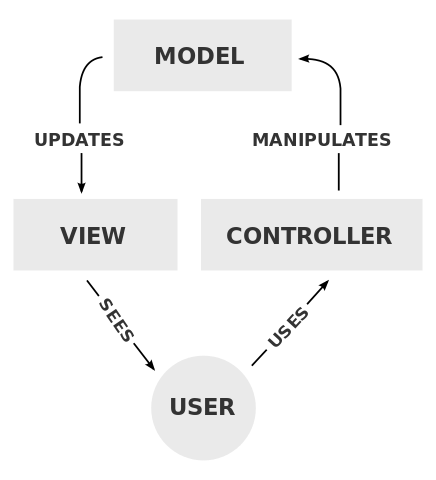
\includegraphics[width=0.35\textwidth]{mvcPattern}
	\caption{Colaborarea între componentele MVC}
\end{wrapfigure}
Alegria a fost implementată cu ajutorul platformei \textbf{Spring Boot} \autocite{SpringBoot}. Platforma a fost aleasă pentru stabilitatea ei excepţională, folosind Spring Framework care stă la baza unora din cele mai mari aplicaţii existente\autocite{springUseCase}, dar şi pentru uşurinţa prin care o aplicaţie poate fi compusă din elemente funcţionale, abstractizând peste nivelele de jos a programului, permiţând alocarea timpului pe logica aplicaţiei, şi nu pe implementarea platformei pe care aplicaţia sa ruleze. Un alt motiv pentru care platforma Spring a fost aleasa, este faptul ca suporta programarea orientată pe aspecte, şi injecţia dependinţelor, permiţând scrierea de cod curat şi uşor de testat.

Cum aplicaţia este bazată pe arhitectura MVC (model-view-controller), aceasta a fost structurată în trei elemente separate: 

\mitem  \textbf{Interfaţa vizuală}: Realizată în \textbf{HTML5}, folosind motorul de templating Thymeleaf pe server şi Bootstrap cu JQuery în client pentru afişarea paginilor. Această combinaţie permite realizarea de pagini cu un aspect modern, responsiv, care funcţionează atât pe ecranul mare al calculatorului, cat şi pe display-ul mic al unui telefon.

\mitem  \textbf{Modele}: O reprezentare a entităţilor din baza de date în sistemul Alegria.

\mitem  \textbf{Controller-e}: Realizează legătura dintre partea vizuala a aplicaţiei şi entităţile din baza de date, asigurând atât metodele care "completează" template-urile cu date, cât şi implementarea interfeţei API care introduce şi extrage date.

\mend

\subsection{Securitate}
Securitatea este un aspect foarte important de luat în considerare, atât pentru accesul la date, cât şi la entităţi. Astfel, în implementare s-a folosit framework-ul \textbf{Spring Security} care uşurează management-ul securităţii, fiind puternic integrat şi cu restul platformei Spring.

Pentru autentificare în vederea utilizării unei resurse protejate, utilizatorul va folosi unul din două mecanisme:
\begin{itemize}
	\item Autentificare securizată prin username şi parolă, aceste detalii fiind stocate în tabela \textit{application\_user}, parola fiind stocata abia după ce a fost trecuta printr-o funcţie criptografica de hashing. Această metodă este folosită pentru autentificarea utilizatorilor în interfaţa de management şi monitorizare. Odată ce procesul a reuşit, un token unic va fi generat, iar request-urile următoare vor fi verificate pe baza procesului descris mai jos.
	\item Autentificare pe baza de token, folosita pentru securizarea API-ului, dar şi în cazul în care un user s-a autentificat deja cu username şi parolă. Fiecare request trebuie sa aibă un token, fie într-un cookie, fie ca parametru în url.
\end{itemize}
Tot în scopuri de securitate, fiecare entitate care poate fi modificata menţine un istoric al tuturor modificărilor, împreuna cu utilizatorul cu care le-a efectuat, iar, pentru o dezvoltare ulterioara, accesul unui utilizator poate fi limitat doar la obiectele care au aceleaşi tag-uri ca şi utilizatorul.
\begin{landscape}
	\begin{figure}
		\centering
		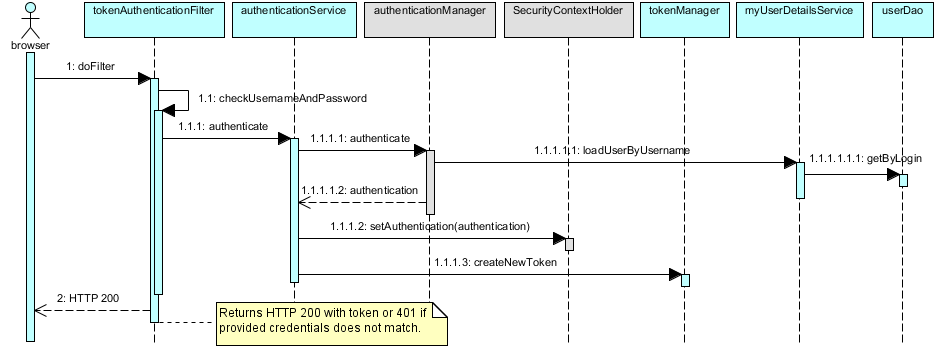
\includegraphics[width=1.75\textwidth, center]{loginUml}
		\caption{Procesul de autentificare în aplicaţie}
		\label{fig:loginUml}
	\end{figure}
\end{landscape}



\subsection{Management}
\begin{figure}[H]
	\centering
	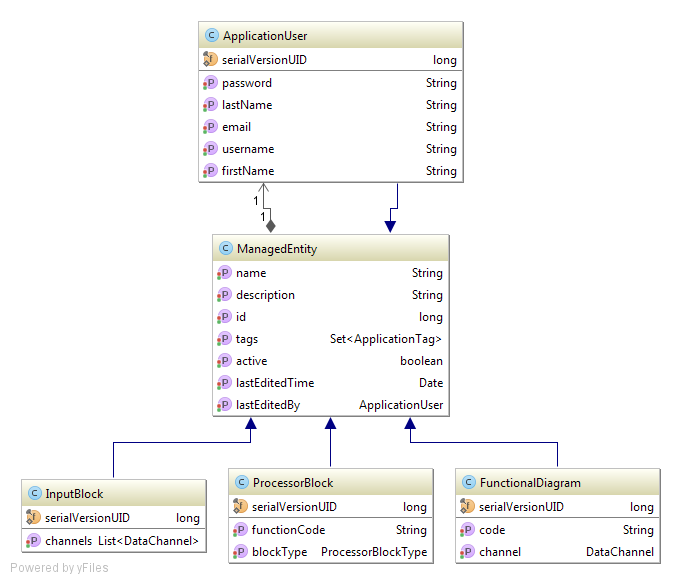
\includegraphics[width=\textwidth, center]{managedEntities}
	\captionsetup{justification=centering}
	\caption{Entităţile care sunt administrate de către utilizator şi implementează \code{ManagedEntity}}
	\label{fig:managedEntities}
\end{figure}
Toate entităţile care implementeaza \code{ManagedEntity} permit apoi operaţii de adăugare, modificare şi ştergere. Acest proces de administrare vizuala foloseşte următoarele resurse:
\begin{itemize}
	\item Un \textbf{repository}, care extinde \code{JpaRepository} din framework-ul Spring Data. Acesta asigură operaţii de căutare, creare, citire, modificare şi ştergere a entităţilor. Un avantaj al folosirii  acestui repository, care implementează paradigma Data Acces Object (DAO) este ca interacţiunea cu baza de date se face într-un mod consistent şi sigur, incompatibilităţile de tip fiind detectate la compilare, şi nu la rulare. În Alegria, toate repository-urile folosite, împreuna cu implementările lor se afla în package-ul \code{ro.pub.acse.sapd.repository}.
	\item O \textbf{vizualizare}, template Thyeleaf, care, într-o singură pagina HTML expune către utilizator toate operaţiile suportate de repository. Aceasta pagina este dinamica, ce foloseşte dialoguri modale încărcate prin AJAX pentru a edita entităţi, fără a fi necesar ca utilizatorul sa fie redirecţionat. Entităţile sunt afişate sub forma tabelară, dinamică, care permite sortarea şi filtrarea după diverse condiţii. Dialogul modal de editare este specific entităţii care este modificate. Vizualizările pentru întreaga lista se afla în \code{resources\textbackslash templates\textbackslash management} iar conţinutul dialogului modal se află în subdirectorul \code{fragments}.
	\item Un \textbf{controller}, clasă cu adnotarea \code{@Controller}, care leagă repository-ul de vizualizare, dar şi specifică către Spring care sunt endpoint-urile (căile pe care acest controller le tratează) prin adnotarea \code{@RequestMapping}. Controllere-le pentru managementul entităţilor se află în \code{ro.pub.acse.sapd.controller.web.management}. Un exemplu de metode care sunt tratate într-un asemenea controller se găsesc în \cref{fig:managementInputs}.
\end{itemize}
\begin{figure}[H]
	\centering
	\captionsetup{justification=centering}
	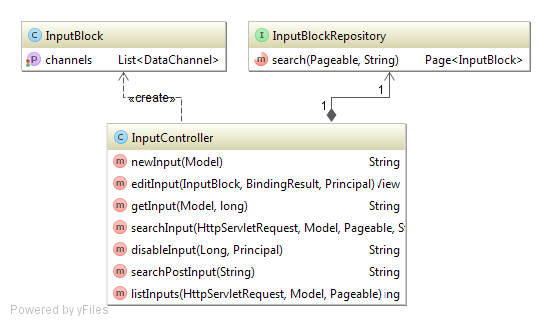
\includegraphics[width=\textwidth, center]{managementInputs}
	\caption{Interacţiunea dintre repository, controller şi entitate}
	\label{fig:managementInputs}
\end{figure}

\subsubsection{Managementul blocurilor de intrare}
Pe lângă elementele descrise mai sus, la management-ul blocurilor de intrare trebuie ca utilizatorul să poată vizualiza şi modifica lista de canale ale unui bloc. În vederea implementării acestei particularităţi, în dialogul modal pentru adăugare şi modificare, a fost realizat un formular dinamic cu câte o line pentru fiecare canal de date. Pentru blocurile de intrare care au deja un canale ataşate, acest formular este generat de către server, în template-ul thymeleaf \code{input.html}, iar, dinamismul formularului este implementat cu ajutorul unor funcţii JavaScript care manipulează structura documentului.
\begin{figure}[H]
	\centering
	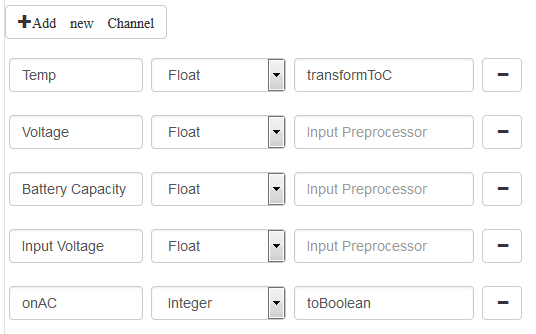
\includegraphics[width=0.8\textwidth, center]{editInput}
	\caption{Formular HTML dinamic pentru editarea canalelor unui bloc de intrare }
	\label{fig:editInput}
\end{figure}
Pentru selectarea blocului de preprocesare a fost folosit endpoint-ul din API de la adresa \code{/blocks/getBlocks} care returnează lista tuturor blocurilor de procesare în format JSON. Această listă este folosită pentru permite completarea automata a câmpului pentru blocul de preprocesare a datelor ale unui canal, folosind librăria JavaScript \textbf{Bootstrap 3 Typeahead} \autocite{typeahead}.

\subsubsection{Managementul blocurilor de procesare}
O particularitate a editării blocurilor de procesare este folosirea librăriei JavaScript \textbf{CodeMirror}\autocite{codemirror} pentru afişarea codului. Cuvintele cheie ale limbajului dat de tipul blocului fiind evidenţiate, acest lucru făcând dezvoltarea codului mult mai facila. Un alt avantaj al acestei librari este posibilitatea găsirii erorilor de sintaxa mult mai rapid, fără a testa blocul. Aceasta funcţionalitate este implementata cu ajutorul unei funcţii care se executa de fiecare dată când valoarea selectată în input-ul "Block Type" se modifică.
\begin{figure}[H]
	\centering
	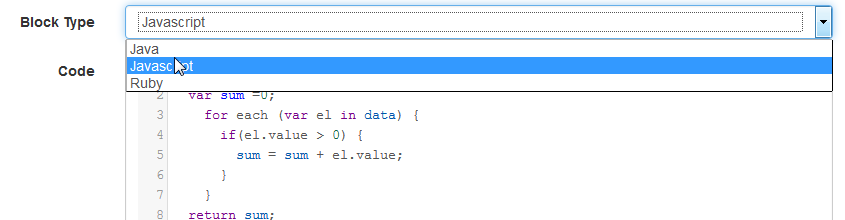
\includegraphics[width=1.2\textwidth, center]{codemirrorExample}
	\caption{Modificarea limbajului din editorul CodeMirror în funcţie de tipul blocului}
	\label{fig:codemirrorExample}
\end{figure}
\subsubsection{Managementul diagramelor}
Pentru implementarea funcţiilor de design vizual al diagramelor funcţionale s-a ales librăria JavaScript \textbf{GoJS} \autocite{gojs}. Aceasta permite implementarea de diagrame interactive, fiind compatibilă cu toate browsere-le cat şi cu dispozitivele mobile moderne. Deoarece asigură suport pentru drag-and-drop, copiere şi lipire, undo şi redo dar şi multe alte funcţionalităţi, librăria reprezinta un punct foarte bun de plecare. Un alt avantaj al acestei librarii este ca suporta adăugarea de condiţii asupra diagramei chiar la construcţia acesteia. Din acest motiv, librăria a fost configurata sa nu permită decât legături de la o ieşire la o intrare.

In vederea realizării acestor configurări fişierul JavaScript \code{diagram.js} a fost scris. Aici sunt configurate tipurile de blocuri:
\begin{itemize}
	\item \textbf{Canale de intrare}: acestea sunt configurate sa nu poată avea intrări, şi doar o singură ieşire. Atunci când un canal de intrare este selectat, utilizatorul poate sa îi atribuie un nume şi să selecteze care este canalul referfeniţat de acel bloc. Aceasta selecţie se face cu ajutorul unui input cu auto completare.
	\item \textbf{Blocuri de procesare}: deoarece numărul de intrări este variabil, funcţia  \code{addPort} a fost implementată. Aceasta este apelata atunci când utilizatorul dă click pe opţiunea "Add input" din meniul contextual al blocului. Pentru operaţiunea de ştergere a portului, funcţia \code{removePort(port)} a fost implementată. Ordinea acestor porturi determină şi ordinea elementelor din lista cu care este apelat blocul de procesare. Atunci acesta este selectat, utilizatorul poate sa îi atribuie un nume şi sa selecteze care este blocul de procesare referfeniţat. Aceasta selecţie se face cu ajutorul unui input cu auto completare. Astfel, acelaşi bloc de procesare poate fi folosit de mai multe ori chiar şi în cadrul aceleiaşi diagrame. Pentru uşurinţă dezvoltării, linkuri către detaliile blocului de procesare sunt disponibile chiar în interiorul diagramei.
	\item \textbf{Final}: bloc ce semnifica canalul de ieşire. Configurat cu un singur port de intrare, el nu poate fi legat decât la o singura ieşire.
	\item \textbf{Comentariu}: nu se poate lega în diagrama şi nu ia parte la execuţia acesteia. 
\end{itemize}
Toate aceste blocuri sunt adăugate şi într-o paleta pentru adăugare uşoară în diagrama. Deoarece blocul "Final" nu poate avea decât o singură instanţă, acesta nu este disponibil în paletă.
\begin{figure}[H]
	\centering
	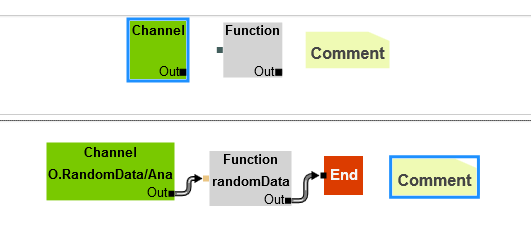
\includegraphics[width=1.2\textwidth, center]{diagramPalleteAndExample}
	\caption{Paleta de blocuri şi exemplu de instanţe ale acestora}
	\label{fig:diagramPalleteAndExample}
\end{figure}
Când utilizatorul salvează o diagramă, un model JSON a acesteia este generat, model ce este apoi salvat în baza de date. În acest model sunt salvate proprietăţile diagramei, urmate de o lista nodurilor, şi nu în ultimul rând legăturile dintre porturile nodurilor.

\subsubsection{Administrare tag-uri}
După cum s-a discutat în secţiunea despre securitate, fiecare entitate care este administrata de utilizator poate avea mai multe taguri. Acestea reprezintă o lista de cuvinte care specifică un concept, spre exemplu, toate entităţile care sunt folosite într-o diagrama pot avea acelaşi tag. Tagurile permit astfel gruparea entităţilor, fiind folosite în căutare.
\begin{figure}[H]
	\centering
	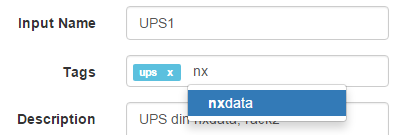
\includegraphics[width=0.7\textwidth, center]{tagsEdit}
	\caption{Editarea tag-urilor unui bloc de intrare}
	\label{fig:tagsEdit}
\end{figure}
Pentru implementare, pe partea de server au fost creata clasa \code{ApplicationTag}, cu doua câmpuri: nume, şi Id. Toate instantele acestei clase sunt salvate în baza de date în tabela \code{application\_tag}, iar endpoint-ul \code{/tags/getTags} întoarce toate tag-urile din acea tabela. Acest serviciu API este folosit de librăria JavaScript Bootstrap Tags Input \autocite{tagsinput}, care, împreună cu librăria de autocompletare \autocite{typeahead}, permite utilizatorului să selecteze taguri deja existente. Atunci când utilizatorul introduce totuşi un tag care nu exista deja în baza de date, acesta este creat automat, fiind setat direct pe entitatea modificată. Fiecare \code{ManagedEntity} are un set de taguri, permiţând salvarea tagurilor în baza de date, într-un tabel separat, care implementeaza relaţia de Multi-la-Multi dintre entitate şi \code{ApplicationTag}.
\begin{figure}[H]
	\centering
	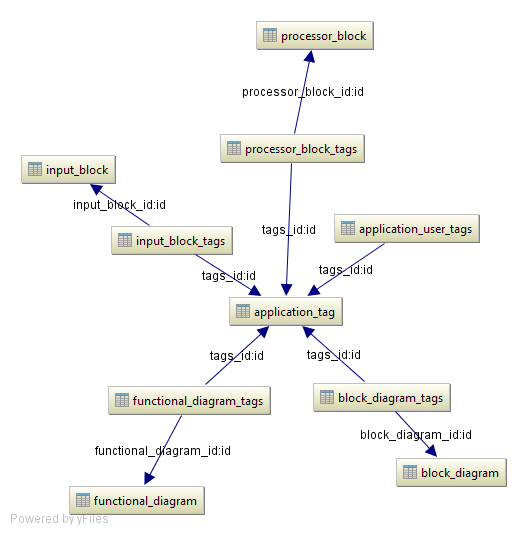
\includegraphics[width=\textwidth, center]{tags}
	\caption{Relaţiile dintre tabela \code{tags} şi celelalte entităţi}
	\label{fig:tags}
\end{figure}
\subsection{Monitorizare}
O chestiune de mare importanta este vizualizarea datelor ce au intrat sau au fost procesate de aplicaţie. În acest scop, a fost implementată vizualizarea datelor în timp real. Pentru extragerea informaţiilor de pe un canal se folosesc endpoint-urile din API de la \code{/api/fetch/{channelId}}, care întorc punctele de pe un canal dintr-un anumit interval de timp, in format JSON.

Deoarece datele procesate de aplicaţie sunt de mai multe tipuri, apare totuşi problema modului lor de afişare. În funcţie de datele întoarse prin API, se selectează unul din doua moduri; Pentru datele numerice, o reprezentare cu ajutorul unui grafic, folosind librăria dygraphs \autocite{dygraphs}, iar pentru datele care nu pot fi reprezentate numeric, acestea sunt afişate tabelar, ca şiruri de caractere.

Pentru ambele moduri de reprezentare, utilizatorul are opţiunea sa obţină doar datele dintr-o anumita perioada de timp, sau chiar ultimele înregistrări pe acel canal. Acest mod de selecţie este ilustrat în \cref{fig:monitorDataFilter}
\begin{figure}[H]
	\centering
	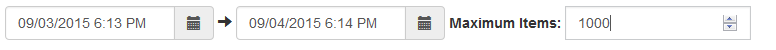
\includegraphics[width=1.2\textwidth, center]{monitorDataFilter}
	\caption{Filtrarea datelor obţinute}
	\label{fig:monitorDataFilter}
\end{figure}
\section{API-ul aplicaţiei}
Pentru a permite interfaţarea aplicaţiei cu alte servicii, dar şi pentru a facilita dezvoltarea unor interfeţe web dinamice, aplicaţia dispune de un API REST. Acesta a fost configurat sa folosească date în format JSON.

În următoarea lista sunt descrise toate endpoint-urile API-ului, împreună cu detalii despre folosirea acestora. În afara de câteva excepţii menţionate, toate aceste servicii folosesc metoda HTTP GET.
\begin{itemize}
	\item \code{/blocks/getBlocks}: întoarce toate blocurile de procesare din baza de date. 
	\item \code{/blocks/getChannels}: întoarce toate canalele declarate în baza de date. Pentru fiecare canal returnat, se specifica de la ce bloc de intrare face parte, sau dacă este ieşirea unui diagrame funcţionale.
	\item \code{/tags/getTags}: întoarce toate tagurile existente în aplicaţie.
	\item \code{/api/put/\{inputId\}/\{channelId\}/\{data\}}: Adaugă punctul \code{data} pe canalul specificat prin \code{channelId}. Datele primite sunt în format \code{String}, care respecta standardul specificat în RFC3986 \autocite{rfc3986}. Foloseşte metoda PUT.
	\item \code{/api/put/openTDSB}: Adaugă date în formatul openTDSB\autocite{openTSDB}. In corpul requestului trebuie să se afle un JSON care respecta standardul impus. Foloseşte metoda PUT.
	\item \code{/api/fetch/\{channelId\}}: Întoarce date de pe canalul \code{channelId}. Următorii parametrii pot fi folosiţi pentru a extrage doar anumite date:
	\begin{itemize}
		\item \code{from}: Data de început a istoricului, în format ISO 8601.
		\item \code{to}: Data de final a istoricului, în format ISO 8601.
		\item \code{maxItems}: Numărul maxim de înregistrări ce sunt returnate. Acest parametru are $500$ ca valoare implicită.
	\end{itemize}
	\item \code{/api/fetch/last/\{channelId\}}: Întoarce date de pe canalul \code{channelId}. Următorii parametrii pot fi folosiţi pentru a extrage doar anumite date:
	\begin{itemize}
		\item \code{maxItems}: Numărul maxim de înregistrări ce sunt returnate. Acest parametru are $500$ ca valoare implicită.
	\end{itemize}
\end{itemize}
Pe lângă aceste metode, aplicaţia mai pune la dispoziţie şi API-ul generat automat cu ajutorul Spring Data. Acesta permite adăugarea, modificarea, ştergerea şi căutarea entităţilor folosite în aplicaţie programatic.

\section{Executarea unui bloc de procesare}
Interacţiunea cu blocurile de procesare se face prin Spring Bean-ul \code{BlockExecutor}. Acesta este responsabil de iniţializarea tuturor implementărilor pentru interfaţa \code{GenericBlockExecutor}. Pentru fiecare implementare există un câmp asociat în enumeraţia \code{ProcessorBlockType}, câmp care este folosit ca proprietate în entitatea \code{ProcessorBlock}. Acest Bean poate fi apoi injectat folosind adnotarea \code{@Autowired} în toate clasele care doresc sa execute blocuri.

Interfaţa \code{GenericBlockExecutor} are o singura metoda \code{processData} cu doi parametrii: unul de tip String, reprezentând codul funcţiei ce trebuie executat, şi unul de tip \code{List<DataPoint>} care conţine toate punctele ce pot fi folosite în blocul respectiv. Clasa \code{DataPoint} are doua câmpuri: valoare şi instanta de timp. Următoarele implementări a interfeţei \code{GenericBlockExecutor} exista în sistem:
\begin{itemize}
	\item \code{JavaBlockExecutor}: Acest executor reprezinta un caz special deoarece foloseşte clase locale, ce sa afla deja în classpath-ul JVM-ului pe care rulează aplicaţia. Aceste blocuri pot fi folosite pentru a extinde aplicaţia cu cod de înaltă performaţă, acţionând ca un mecanism de extensii ale aplicatei, permiţând interacţiunea cu alte sisteme. Aceste blocuri pot sa reprezinte doar o interfaţa pentru apelul unor librarii externe, făcând posibilă, spre exemplu, implementarea unui bloc care să execute scripturi MATLAB.
	Acest bloc primeşte ca parametru doar numele canonic al clasei, iar, la execuţie încarcă clasa referentiată folosind funcţii din pachetul \code{java.lang.reflect}. Dacă clasa nu este găsită, sau o eroare are loc la execuţia clasei, o excepţie de tipul \code{BlockExecutionException} este generată.
	\begin{figure}[H]
		\centering
		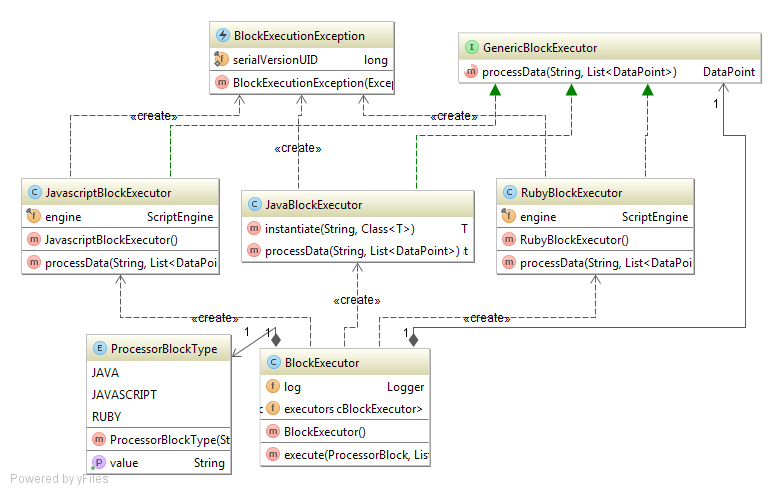
\includegraphics[width=1.3\textwidth, center]{blockExecutors}
		\caption{Clasele ce asigura executarea unei diagrame}
		\label{fig:blockExecutors}
	\end{figure}
	\item \code{JavascriptBlockExecutor}: Executor ce poate rula cod JavaScript pe server. Aceste blocuri trebuie sa conţină o funcţie \code{parseInput} care ia ca parametru o lista de \code{DataPoint}. Pentru execuţia blocurilor de acest tip, standardul JSR 223 \autocite{JSR223} vine în ajutor prin abstractizarea funcţionalităţii interne necesare execuţiei de cod scris într-un limbaj dinamic, direct în maşina virtuala Java. In versiunea 8 a JVM-ului aceste funcţii sunt executate folosind runtime-ul de înaltă performantă Nashorn, care este accelerat de modificări recente, introduse în JSR 292  \autocite{JSR292}, ridicând performanta codului JavaScript la un nivel apropiat de funcţiile scrise în Java. Pentru versiunile precedente de JVM este folosit Mozilla Rhino. Dacă funcţia \code{parseInput} nu este găsită, sau o eroare are loc la execuţia script-ului, o excepţie de tipul \code{BlockExecutionException} este generată. Scriptul poate returna direct instante ale interfeţei \code{DataPoint}, sau alte obiecte care sunt apoi reprezentate ca un \code{StringDataPoint}.
	
	\item \code{RubyBlockExecutor}: Executor ce rulează cod Ruby pe server. Din punct de vedere al implementării este similar cu \code{JavascriptBlockExecutor}, însă foloseşte librăria JRuby \autocite{jruby} .
	
\end{itemize}

\section{Executarea unei diagrame funcţionale}
\Cref{fig:intrareDate} prezintă şi modul în care o diagrama este executată. Diagramele sunt lansate în execuţie de fiecare dată când un canal folosit în ea primeşte informaţii noi. Dacă doua canale primesc date în acelaşi timp, atunci diagrama va fi lansată în execuţie tot de doua ori, pentru ambele puncte de date primite.

\subsection{Ordinea execuţiei blocurilor}
Problema ordinii execuţiei unei FBD este intens dezbătută atât în literatura, cat şi în aplicaţiile industriale. Cum standardul \textit{IEC61131-3} \autocite{IEC61131-3} nu propune o soluţie pentru ordinea de execuţie, producătorii industriali folosesc metode proprii, de la separarea blocurilor într-un tabel şi executarea de la stânga la dreapta, sus în jos \autocite[11]{TM241}, la definirea manuala a ordinii execuţiei \autocite[11]{Logix5000} sau folosind algoritmi care determina automat ordinea de execuţie \autocite[5]{GEFANUC}.

În implementarea din Alegria s-a ales proiectarea unei metode automate pentru depistarea ordinii în care diagrama trebuie executata. Deoarece aceasta reprezinta un graf aciclic orientat, prima etapa a execuţiei este transformarea într-un graf reprezentat prin lista de adiacenta, unde fiecare bloc de intrare, bloc şi de procesare reprezinta un nod. Din aceasta reprezentare se omit blocurile de comentarii. Odată ce transformarea a fost efectuata cu succes, se încercă aplicarea unui algoritm de sortare topologică\autocite{toposort} a grafului obţinut. Aceasta implică găsirea unei ordini astfel încât, pentru orice arc orientat $uv$ de la  $u$ la $v$, $u$ este înaintea lui $v$. 
Matematic problema poate fi formulata astfel:

\begin{definition} 
	O \textbf{ordine topologica}, notata $ord_D$, au unui graf orientat aciclic $D = (V,E)$ atribuie fiecărui nod o valoare astfel încât $ord_D(x) < ord_D(y)$ pentru orice arc $ x \rightarrow y \in E$.
\end{definition}
Mai multi algoritmi pentru efectuarea unei asemenea sortări exista în literatura \autocite{toposortArticle}, însa, deoarece grafurile în discuţie sunt statice, la care nu se adaugă sau şterg noduri, s-a ales un algoritm clasic, stabil din punct de vedere numeric descris de Kahn în 1962 \autocite{topoKahn}.

Simplificat, algoritmul implementat urmăreşte următorii paşi:
\begin{enumerate}
	\item Identifică toate nodurile spre care nu vine nici un arc. Valoarea acestor noduri va fi $0$. In cazul diagramelor, este vorba de toate canalele de intrare, şi de blocurile de procesare care nu au nici o intrare. Dacă aceste noduri nu există, înseamnă ca graful nu respecta condiţia de graf aciclic, deci acesta nu va putea fi executat.
	\item Se alege unul din nodurile găsite mai sus.
	\item Se şterge acest nod de valoare zero, împreună cu toate arcele care ies din el.
	\item Se repeta paşii 1 şi 2 pana când nu mai exista noduri în graf.
\end{enumerate}
Algoritmul descris mai sus rulează în $\mathcal{O}(V + E)$. 

\begin{algorithm}[H]
	\KwData{Un graf orientat acliclic reprezentat prin lista de adiacenta}
	\KwResult{Lista nodurilor ordonate topologic}
	$L \gets$ Lista goala ce va conţine nodurile sortate \;
	$S \gets$ Lista tuturor nodurilor spre care nu exista nici un arc \;
	\While{ $S$ conţine elemente }{ 
		şterge nodul $n$ din $S$ \;
		introdu nodul $n$ în $L$ \;
		\ForEach{nod $m$ care are un arc $e$ de la $n$ la $m$}{
			şterge arcul $e$ din graf\;
			\If{$m$ nu mai are arce spre el}
			{inserează $m$ în $S$}
		}{
	} 
	
}
\eIf{mai exista arce în graf}
{\Return{\textbf{Eroare:} Graful are cel puţin un ciclu}}{
	{\Return{$L$ (graful sortat topologic)}}
}
\label{alg:khan}
\caption{Algoritmul lui Khan pentru sortare topologică}
\end{algorithm}

Astfel, pentru diagrama din \cref{fig:exempluDiagrama}, o posibila ordine de execuţie este descrisă în \cref{fig:executionOrder}.
\begin{figure}[H]
	\centering
	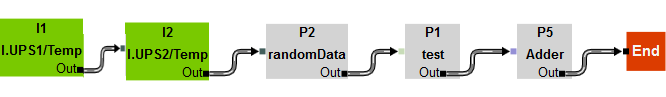
\includegraphics[width=\textwidth]{diagramExecutionOrder}
	\caption{Ordinea execuţiei pentru diagrama din \cref{fig:exempluDiagrama}}
	\label{fig:executionOrder}
\end{figure}
După cum se observă în \cref{alg:khan}, acesta poate detecta grafuri care conţin cicluri şi nu pot fi rezolvate. Aceasta verificare permite detectarea erorilor, precum cea din diagrama \ref{fig:badDiagram}, şi informarea utilizatorului pentru ca acesta să rezolve problema.
\begin{figure}[H]
	\centering
	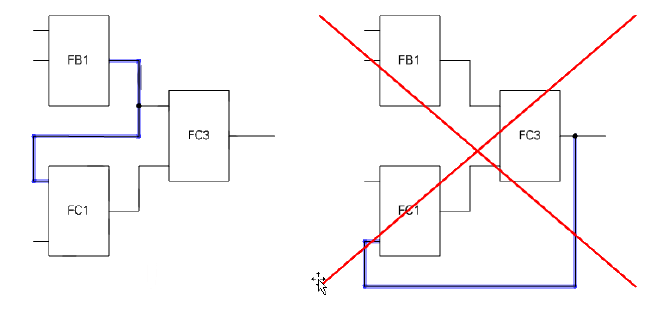
\includegraphics[width=0.95\textwidth]{badDiagram}
	\caption{Diagramă ce conţine cicluri}
	\label{fig:badDiagram}
\end{figure}

Deşi ciclurile la nivel de diagrama nu sunt permise, cele la nivel de canal sunt. Astfel, ieşirea unei diagrame poate fi setata ca intrare pentru aceeaşi diagrama, permiţând executarea în bucla, deoarece odată ce o diagrama se termina de executat şi salvează rezultatul pe canal, aceasta se relansează în execuţie cu noi informaţii. Cu astfel de bucle se poate implementa diagrame ce interacţionează intre ele. Un alt aspect pozitiv al faptului ca intrările unor diagrame pot fi ieşirile unor alte diagrame este faptul ca procese foarte complexe pot fi descompuse în părţile componente prin simpla înlănţuire a diagramelor.

\subsection{Generarea rezultatului}
Odată ce ordinea de execuţie a fost calculată, procesul de calcul al rezultatului este destul de simplu, fiind ilustrat în \cref{alg:executeDiagram}:

\begin{algorithm}[H]
	\KwData{Lista nodurilor ordonate topologic}
	\KwResult{Punctul de date ce trebuie adaugat pe canalul de iesire a diagramei}
	$rezultate \gets$ Relaţie cheie-valoare intre nod şi rezultatul execuţiei lui\;
	$L \gets$ Lista ce conţine nodurile sortate \;
	\ForEach{nod $m$ din $L$}{
		$intrari \gets$ Lista goala de intrări pentru nodul $m$ \;
		\ForEach{arc de la $n$ către $m$}{
			\eIf{In $rezultate$ exista rezultatul pentru blocul $n$}
			{Adaugă în $intrari$ valoarea de la $rezultate(n)$\;}{
				{\Return{\textbf{Eroare:} Graful nu poate fi executat\;}}
			}	
		}
		\eIf{$m$ este un bloc de procesare}
		{Executa blocul folosind intrările $intrari$\;
			Adaugă în $rezultate$ valoarea calculata\;}{
			\ElseIf{$m$ este un canal de date} {
				Adaugă în $rezultate$ ultima valoare de pe canal\;}
		} 
	}
	
	{\Return{Ultima valoare din $rezultate$}}
	\label{alg:executeDiagram}
	\caption{Execuţia unei diagrame FBD}
\end{algorithm}

\subsection{Implementarea în Aplicaţie}
Pentru execuţia diagramelor este folosit Spring Bean-ul \code{DiagramExecutor}. Acesta este responsabil atât de parsarea unei diagrame cât şi de execuţia şi extragerea rezultatelor. Acest Bean poate fi apoi injectat folosind adnotarea \code{@Autowired} în toate clasele care doresc sa execute diagrame.

Parsarea este realizata cu ajutorul interfeţei \code{DiagramParser}, aceasta permiţând transformarea diagramei într-un graf reprezentat prin listă de adiacenţă. O implementarea a acestei interfeţe este clasa \code{GoJsDiagramParser} care parsează JSON-ul generat de librăria GoJS. Aceasta parsare se face cu ajutorul librăriei Jackson, folosind modelul de date din figura \cref{fig:gojsdiagramModel}. Dacă parsarea nu este realizata cu succes, atunci o excepţie de tipul \code{DiagramParseException} este aruncată.
Dacă se doreşte înlocuirea librăriei de front-end pentru realizarea diagramelor, sistemul poate fi adaptat doar prin scrierea unei noi clase ce implementează \code{DiagramParser}.

\begin{figure}[H]
	\centering
	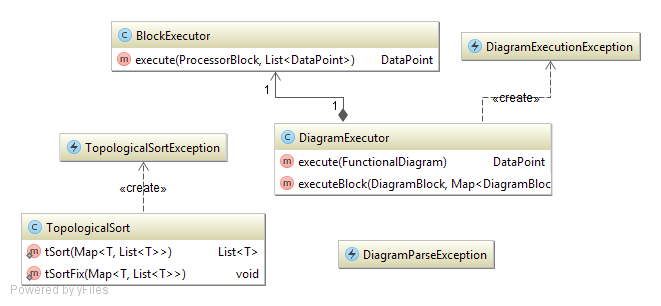
\includegraphics[width=\textwidth, center]{diagramExecuteClasses}
	\caption{Clasele implicate în executarea unei diagrame}
	\label{fig:diagramExecuteClasses}
\end{figure}
Odată ce parsarea a fost efectuată, execuţia blocului poate continua: folosind clasa \code{TopologicalSort}, o implementare a \cref{alg:khan} cu tipuri generice şi expresii lambda, ordinea de execuţie este calculată. Apoi, \cref{alg:executeDiagram} este executat, si, cu ajutorul bean-ului \code{BlockExecutor} blocurile din diagrama sunt executate. Rezultatul final al metodei \code{execute} este un \code{DataPoint} care va fi salvat în baza de date, pe canalul de ieşire a diagramei.

O alta chestiune importantă este determinarea momentelor când o diagrama trebuie executată. În acest scop, pe fiecare canal se stochează o mulţime de diagrame care trebuie lansate atunci când se primesc informaţii noi. Această listă este actualizată de fiecare data când diagrama se modifică prin interfaţa web. Metodele din \code{DiagramParser} sunt folosite pentru a obţine lista de canale utilizate şi pe fiecare dintre acestea, pe proprietatea \code{Set<FunctionalDiagram> subscribedDiagrams} este adăugată acea diagrama. Pentru a nu se pierde consitenţa datelor, cât timp diagrama este modificată, ea nu se mai poate lansa în execuţie.
\begin{figure}[H]
	\centering
	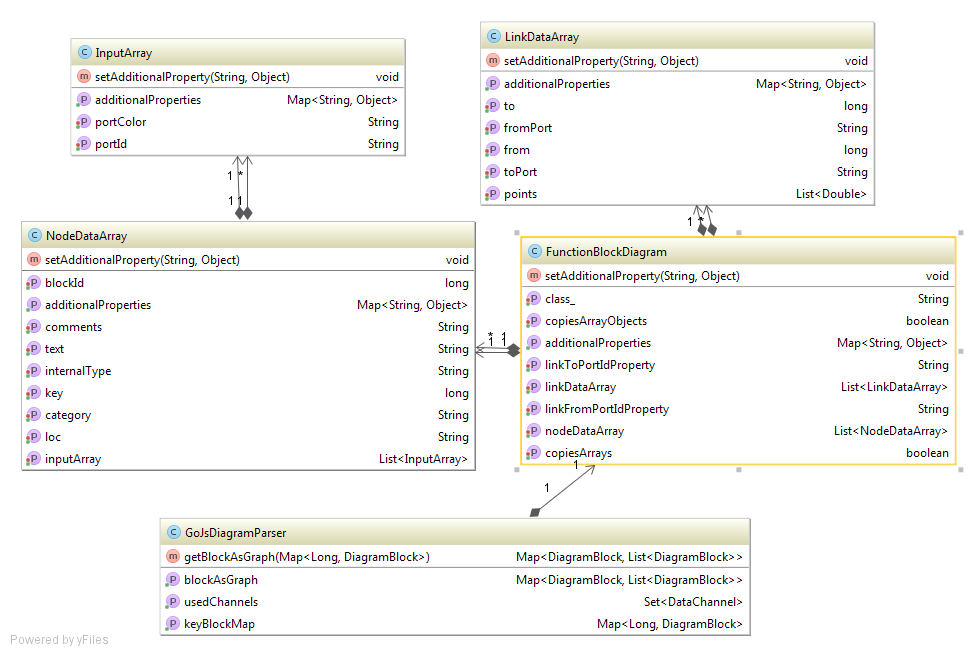
\includegraphics[width=1.2\textwidth, center]{gojsdiagramModel}
	\caption{Modelul de date pentru diagramele GoJS}
	\label{fig:gojsdiagramModel}
\end{figure}
\section{Serviciul de date}
Serviciul de date, implementat prin Spring Bean-ul \code{DataService} permite abstractizarea modului în care \code{DataPoint}-urile sunt scrise în baza de date. În această implementare, datele sunt stocate în aceeaşi instanta de PostgreSQL ca şi entităţile. Aceasta clasa foloseşte interogări SQL optimizate pentru a fi executate cat mai rapid, prin stocarea acestora direct pe serverul SQL.
\begin{figure}[H]
	\centering
	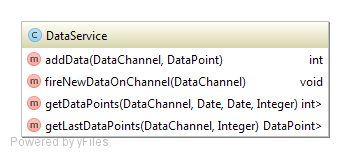
\includegraphics[width=0.6\textwidth, center]{dataService}
	\caption{Interfaţa aplicaţiei cu baza de date pentru informaţii}
	\label{fig:dataService}
\end{figure}
Această clasă asigură şi execuţia diagramelor din lista de \code{subscribedDiagrams} a canalului ce primeşte date. Această execuţie se executa în mod \textbf{asincron}, pentru a nu bloca firul de execuţie care primeşte date. Asincornicitatea este implementata printr-un pool de thread-uri care primesc task-uri de execuţie, thread-ul apelant nefiind interesat de rezultatul execuţiei. Astfel, putem considera că implementarea pe mai multe fire de execuţie este de tipul fire-and-forget.

Pentru a garanta o metoda de management a firelor de execuţie, s-au folosit capabilităţile native ale platformei Spring \autocite{springAsync} , prin adnotarea \code{@Async}.
\section{Baza de date}

După cum s-a discutat în capitolul despre arhitectura, aplicaţia are nevoie de mijloace de stocare pentru două tipuri de date: modelul entităţilor, şi datele primite şi procesate.
\subsection{Stocarea entităţilor} 
Petru stocarea entităţilor au fost investigate mai multe opţiuni de baze de date relaţionale, PostgreSQL fiind aleasă pentru stabilitatea şi posibilitatea de replicare volumelor mari de date, dar şi pentru uşurinţa extensibilităţii\autocite{postgresql}. Un alt avantaj al folosirii PostgreSQL este lipsa costului licenţei, întrucât este o aplicaţie open-source cu o comunitate foarte dinamică.
\begin{landscape}
	\begin{figure}
		\centering
		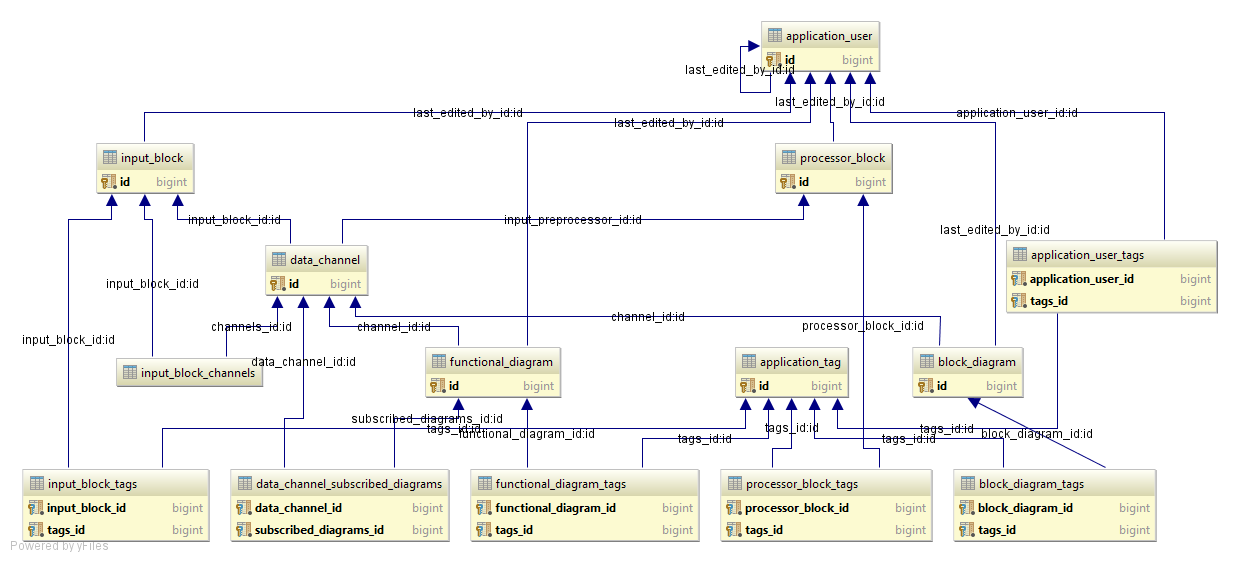
\includegraphics[width=1.8\textwidth]{dbDiagram}
		\caption{Modelul entităţilor din baza de date}
		\label{fig:dbDiagram}
	\end{figure}
\end{landscape}

Pentru generarea schemei bazei de date s-a folosit ORM-ul implicit din Spring Data, Hibernate \autocite{hibernate} . Acesta permite generarea schema unei baze de date cu ajutorul programării orientate pe aspecte, prin adăugarea de adnotări pe clase Java. Această generare se realizează automat, de fiecare dacă când modelul Java se modifica.
\begin{figure}[H]
	\centering
	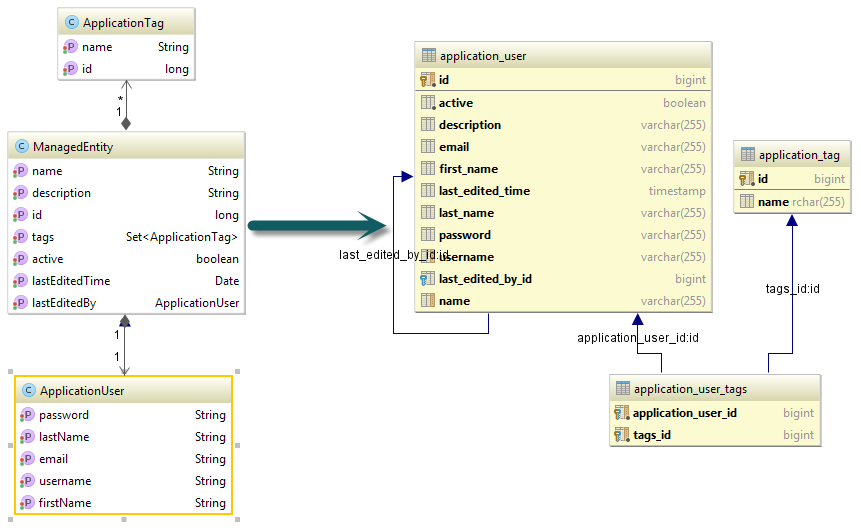
\includegraphics[width=\textwidth]{ORMtransform}
	\captionsetup{justification=centering}
	\caption{Transformarea claselor Java în relaţii din baza de date prin intermediul unui ORM}
	\label{fig:ORMtransform}
\end{figure}


